% 2011 年江西卷理科第 10 题：小圆沿大圆内壁滚动，M、N 的轨迹选项。
% 来源 PDF：普通高考/2011/2011江西理.pdf，SHA-256 9fa84ea67ec469ea2a8bb4a06f9d79b6c5a94e8b08a52d2045e30daabf8d1582。
% 原页：第 1 页第 2 栏上部，书页码 677。上图为滚动示意；下排为 A—D 四个轨迹选项（示意）。
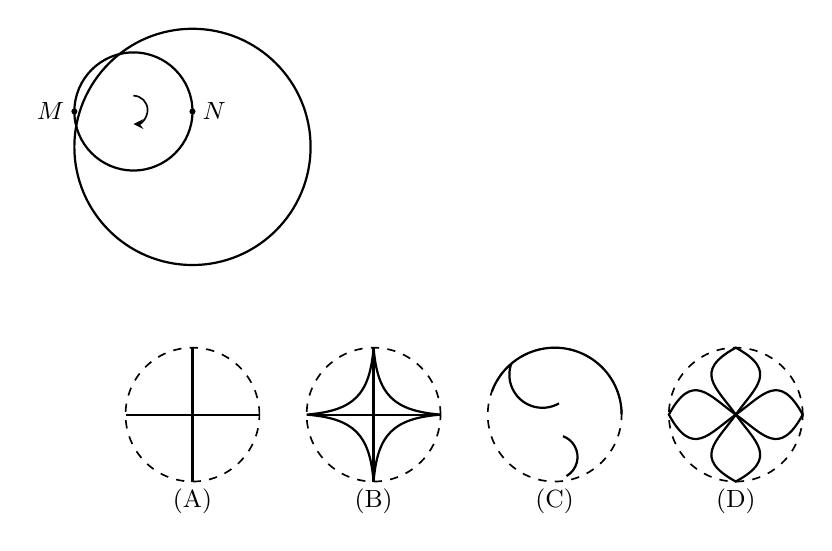
\begin{tikzpicture}[>=stealth, semithick, font=\small]
  % 滚动示意
  \draw[thick] (0,0) circle (1.5);
  \draw[thick] (-0.75,0.45) circle (0.75);
  \draw[->] (-0.75,0.45) ++(0.0,0.2) arc (90:-90:0.18);
  \fill (-1.5,0.45) circle (1.1pt) node[left] {$M$};
  \fill (0.0,0.45) circle (1.1pt) node[right] {$N$};
  % 四个选项
  \begin{scope}[yshift=-3.4cm]
    \draw[dashed] (0,0) circle (0.85);
    \draw[thick] (-0.85,0)--(0.85,0);
    \draw[thick] (0,-0.85)--(0,0.85);
    \node at (0,-1.1) {(A)};
  \end{scope}
  \begin{scope}[xshift=2.3cm, yshift=-3.4cm]
    \draw[dashed] (0,0) circle (0.85);
    \draw[thick] (0.85,0) .. controls (0.25,0.05) and (0.05,0.25) .. (0,0.85)
      .. controls (-0.05,0.25) and (-0.25,0.05) .. (-0.85,0)
      .. controls (-0.25,-0.05) and (-0.05,-0.25) .. (0,-0.85)
      .. controls (0.05,-0.25) and (0.25,-0.05) .. (0.85,0);
    \draw[thick] (-0.85,0)--(0.85,0);
    \draw[thick] (0,-0.85)--(0,0.85);
    \node at (0,-1.1) {(B)};
  \end{scope}
  \begin{scope}[xshift=4.6cm, yshift=-3.4cm]
    \draw[dashed] (0,0) circle (0.85);
    \draw[thick] (0.85,0) arc (0:160:0.85);
    \draw[thick] (-0.55,0.65) arc (160:300:0.42);
    \draw[thick] (0.15,-0.78) arc (300:430:0.28);
    \node at (0,-1.1) {(C)};
  \end{scope}
  \begin{scope}[xshift=6.9cm, yshift=-3.4cm]
    \draw[dashed] (0,0) circle (0.85);
    \foreach \a in {0,90,180,270}{
      \begin{scope}[rotate=\a]
        \draw[thick] (0,0) .. controls (0.35,0.25) and (0.55,0.55) .. (0.85,0.0)
          .. controls (0.55,-0.55) and (0.35,-0.25) .. (0,0);
      \end{scope}
    }
    \node at (0,-1.1) {(D)};
  \end{scope}
\end{tikzpicture}
